\chapter{The KLOE and J-PET detectors}
\label{chapter:detectors}

This Thesis covers two approaches to searching for violations of the symmetry under reversal in time: a comparison of probabilities for A$\to$B and B$\to$A transitions in the system of quantum-entangled neutral K mesons and a determination of the expected value of a \Ts-odd operator constructed using angular correlations between photons from an ortho-positronium decay. The former is performed using the KLOE experimental setup, constituted by a large general-purpose particle detector recording the decays of $\phi$ mesons into kaons, taking place in electron-positron collisions at 1 GeV energy scale. The latter will be realized with the J-PET detector, a device dedicated to recording photons from electron-positron annihilation and positronium atom decays, at low energies of positron thermalization in matter.

Although these two measurements are based on substantially different principles and are conducted in very different conditions, the physical processed involved in these experiments and the setups used to record them are not without similarities. Not only do they both use an electron-positron system to produce a desired physical state, but also both these measurements involve a decay of a neutral state into several photons, where the decay location must be reconstructed in order to calculate event properties essential for the experiment. In each case, reconstruction is performed using the same technique. Application of the same reconstruction scheme in the KLOE and J-PET experimental setups alike was possible due to several properties shared by them in terms of recording neutral particle decays into photons.

This Chapter presents details of the KLOE and J-PET detectors used in the studies covered by this Thesis, with a special emphasis on the links between them which made it possible to employ the same reconstruction algorithm (described in detail in Chapter~\ref{chapter:gps}) in each of these detectors.

\section{The KLOE detector and the DA$\Phi$NE $\phi$-factory}
% The KLOE experimental setup was designed with a primary goal to probe direct \CPs~violation in the decays of neutral K mesons by measurement of the $\Re\left(\frac{\epsilon'}{\epsilon}\right)$ parameter through the following observable double ratio:
% \[ R = \frac{\Gamma(\Ks\to\pi^0\pi^0)\Gamma(\Kl\to\pi^+\pi^-) }{\Gamma(\Ks\to \pi^+\pi^-)\Gamma(\Kl\to\pi^0\pi^0)}, \]
% at the same time allowing for a broad range of other studies in the field of kaon physics~\cite{Campana:1997ai}.
With a broad range of studies of the physics of neutral K meson system as one of its major goals, the properties of the KLOE (K LOng Experiment) detector have been largely dictated by requirements to record the decays of both the short and long-lived neutral kaons with high efficiency. The same reasons influenced the location of KLOE to be at the DA$\Phi$NE $e^+e^-$ collider which provides it with copious pairs of both neutral and charged kaons, produced in the decays of $\phi$ mesons. Next Section presents details of this collider relevant for the studies presented in this work, whereas in the further Sections the features of the KLOE detector are discussed.

%%%%%%%%%%%%%%%%%%%%%%%%%%%%%%%%%%%%%%%%%%%%%%%%%%%%%%%%%%%%%%%%%%%%%%%%%%
% DAFNE                                                                  %
%%%%%%%%%%%%%%%%%%%%%%%%%%%%%%%%%%%%%%%%%%%%%%%%%%%%%%%%%%%%%%%%%%%%%%%%%%
\subsection{The DA$\Phi$NE collider}
\label{sec:dafne}

DA$\Phi$NE, whose name is an acronym for Double Annular $\Phi$-factory for Nice Experiments, is an electron-positron collider operating since 1999 in the National Laboratories of Frascati (LNF) located near Rome, Italy. The whole accelerator complex of LNF is schematically presented in Figure~\ref{fig:dafne}. A linear accelerator (LINAC) provides electron and positrons (where the latter are obtained with conversion of 250 MeV electrons on a metallic target) in 10~ns pulses with a frequency of 50 Hz~\cite{Vignola:1996mt}. Subsequently, both electrons and positrons are transferred to an accumulator ring where they are cooled in order to damp the emittances of the beams before their injection into DA$\Phi$NE. Finally, electrons and positrons are injected in turns into the storage rings of DA$\Phi$NE as a single bunch at a time.

\begin{figure}[h!]
  \centering
  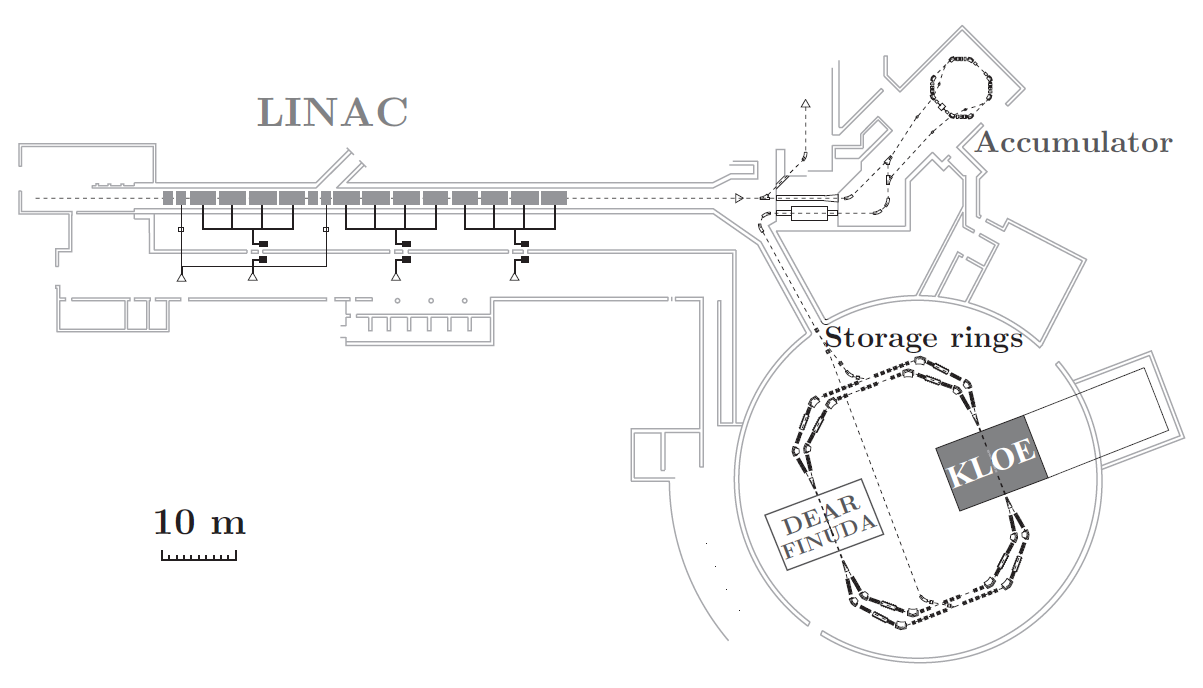
\includegraphics[width=0.7\textwidth]{Chapter3_detectors/img/dafne}
  \caption{Scheme of the acelerator complex of National Laboratories of Frascati which includes the two storage rings of the DA$\Phi$NE collider. Figure adapted from~\cite{kloe_results}.\label{fig:dafne}}
\end{figure}

In order to reduce beam-beam interactions, the DA$\Phi$NE collider consists of separate storage rings for $e^-$ and $e^+$, which intersect at an angle of 25 mrad in two interaction regions. One of them is occupied in turns by the KLOE and SIDDHARTA~\cite{CurceanuPetrascu:2007zz} detectors, while the other served the DEAR~\cite{Lucherini:2003fk} and FINUDA~\cite{Agnello:2007rk} experiments. KLOE, which is of interest in this work, surrounds its interaction region and is oriented so that its $x$ axis is horizontal and perpendicular to the beam direction, $y$ axis is vertical whereas the $z$ axis of the detector frame of reference is parallel to bisector of an angle between the beams.

\begin{table}[h!]
  \centering
  \caption{Selected parameters of the DA$\Phi$NE collider~\cite{Vignola:1996mt}.\label{tab:dafne}}
  \begin{tabular}{cc r}
    \toprule
    \multicolumn{2}{l}{DA$\Phi$NE property} & value \\
    \midrule
    \multicolumn{2}{l}{beam energy} & 510 MeV \\
    \multicolumn{2}{l}{RF frequency} & 368.25 MHz \\
    \multicolumn{2}{l}{inter-bunch-crossing period} & 2.72 ns \\
    \multicolumn{2}{l}{bunches per beam} & 120 \\
    \multicolumn{2}{l}{particles per bunch} & 8.9$\times 10^{10}$ \\
    \multirow{3}{*}{bunch spread}           & $\sigma_x$ & 0.02 cm \\ 
    \multirow{3}{*}{} & $\sigma_y$ & 0.002 cm \\ 
    \multirow{3}{*}{}           & $\sigma_z$ & 3 cm \\
    \multicolumn{2}{l}{bunch crossing angle} & 25 mrad \\
    \bottomrule
  \end{tabular}
\end{table}

The storage rings of the collider contain a total of 120 particle bunches and operate at a RF frequency of 368.25 MHz, which results in an interval of 2.72 ns between subsequent bunch crossings in an interaction region. A single bunch, consisting of about $9\times10^{10}$ electrons or positrons, has a very small spatial spread in the $y$ (vertical) direction perpendicular to the storage ring plane, and is largest in the longitudinal direction ($z$), where its spread reaches 3 cm ($\sigma$). A summary of the DA$\Phi$NE parameters is given in~\tref{tab:dafne}.

The energies of electron and positron beams circulating in DA$\Phi$NE are symmetrical and chosen so as to obtain a center-of-mass energy of the collisions equal to the mass of the $\phi$ meson, i.e.~$\sqrt{s}\approx m_{\phi}=1019.46\pm0.016$ MeV. Thus, in the $e^+e^-$ collisions, $\phi$ mesons are predominantly produced with a cross section of about 3.1 $\mu$b, due to which fact the name of a $\phi$-factory is often attributed to DA$\Phi$NE\@. In fact, during the operation of the KLOE experiment at this collider, a total of about $10^{10}$ of $\phi$ mesons were produced and their decays recorded by KLOE\@.

Due to the small crossing angle of the colliding beams, the produced $\phi$ mesons are almost at rest ($\beta_{\phi}\approx 0.015$) with only a small momentum component in the $x$ direction:
\begin{equation}
  \label{eq:phi_px}
  p_x^{\phi} = 13.1 \ \text{MeV/c}.
\end{equation}

Strong interactions governing the $\phi$ decays make them almost immediately ($\tau_{\phi} = 1.5500\pm0.0058\times 10^{-22}$ s~\cite{pdg2016}) produce a pair of either neutral or charged K mesons or hadronic states such as $\rho\pi^0$, with branching fractions presented in~\tref{tab:phi_brs}.

\begin{table}[h!]
  \centering
  \caption{Branching fractions of major decays of the $\phi$ meson~\cite{pdg2016}.}\label{tab:phi_brs}
  \begin{tabular}{c c}
    \toprule
    Decay & Branching fraction \\
    \midrule
    $\phi\to\mathrm{K}^+\mathrm{K}^-$ & 48.9$\pm$0.5\% \\
    $\phi\to\kaon\akaon$ & 34.2$\pm$0.4\% \\
    $\phi\to\rho\pi^0/\pi^+\pi^-\pi^0$ & 15.32$\pm$0.32\% \\
    \bottomrule
  \end{tabular}
\end{table}

%%%%%%%%%%%%%%%%%%%%%%%%%%%%%%%%%%%%%%%%%%%%%%%%%%%%%%%%%%%%%%%%%%%%%%%%%%
% KLOE                                                                   %
%%%%%%%%%%%%%%%%%%%%%%%%%%%%%%%%%%%%%%%%%%%%%%%%%%%%%%%%%%%%%%%%%%%%%%%%%%
\subsection{General properties of the KLOE detector}
\label{sec:kloe}

The design of KLOE follows a general scheme often used in general purpose particle detectors, with a cylindrical tracking device symmetrically surrounding the interaction region enclosed by a calorimetric detector. However, the properties of these components are specifically driven by the aim to capture a large part of decays of the $\Kl$ meson (whose mean free path in the KLOE conditions is about 3.4 m~\cite{LeeFranzini:2007hj}), minimize kaon regeneration and register photons from hadronic decays into neutral pions.

\begin{figure}[h!]
  \centering
  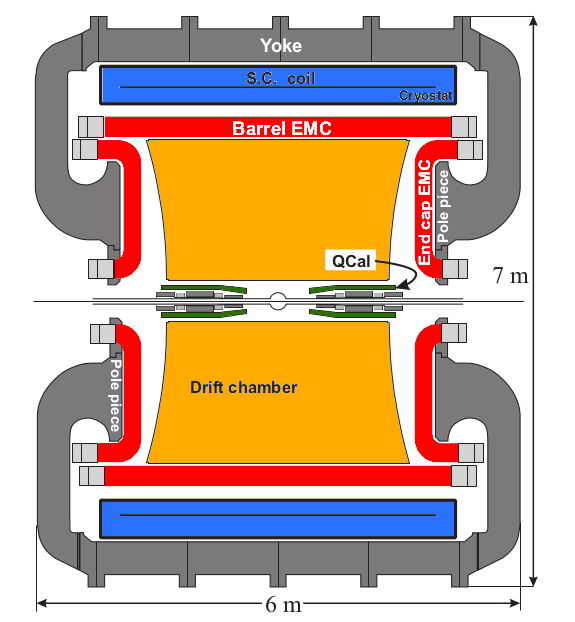
\includegraphics[width=0.6\textwidth]{Chapter3_detectors/img/kloesection2}
  \caption{Longitudinal cross section of the KLOE detector. Its main components comprise a drift chamber~(orange), electromagnetic calorimeter~(red), two calorimeters surrounding quadrupole beam-focusing magnets (green) and a superconducting solenoid~(blue). Figure adapted from~\cite{LeeFranzini:2007hj}.\label{fig:kloe}}
\end{figure}

Figure~\ref{fig:kloe} shows a longitudinal section of the detector. Around the interaction region of DA$\Phi$NE, located in the geometrical center of KLOE, the beam pipe is specially shaped as a sphere of 10 cm radius (which corresponds to about 17$\lambda_{K_S}$ where $\lambda_{K_S}=\beta_{K_S}c\tau_S$) and made of a light Al-Be alloy of 1 mm thickness in order to reduce the probability of neutral kaon regeneration due to nuclear interactions in the beam pipe material. Further from the interaction region, two final focusing quadrupole magnets of the collider are surrounded with tile calorimeters (QCal, marked green in~\fref{fig:kloe}) which decrease the loss of registration of photons from the $\Kl\to 3\pi^0\to 6\gamma$ decays going into the volume of the magnets~\cite{Adinolfi:2002me}.

Most of the KLOE detector volume is filled by a cylindrical drift chamber (DC, marked orange in~\fref{fig:kloe}) whose tracking and particle identification capabilities are aided by the presence of 0.52~T magnetic field directed along the $z$ axis and provided by a superconducting coil (marked blue in~\fref{fig:kloe}). The drift chamber is surrounded by an electromagnetic calorimeter (EMC, red in~\fref{fig:kloe}) which records interactions of photons and other particles. Good hermeticity of the EMC is ensured by its composition of a barrel-shaped part and a set of C-shaped endcaps. As the drift chamber and electromagnetic calorimeter of KLOE are essential for the work presented in this Thesis, they will be discussed in detail in the following Sections.

\subsection{The KLOE drift chamber}
\label{sec:dc}
The tracking of charged particles in KLOE is provided by a large drift chamber shaped as a cylinder with a 2~m outer radius and length of 3.3~m. Such a large sensitive volume allows it to record about \SI{40}{\percent} of decays of the long-lived neutral K mesons before they leave the detector~\cite{LeeFranzini:2007hj}. The region close to the axis of the chamber is hollow up to an inner radius of 25~cm to allow space for the spherical beam pipe, beam-focusing magnets and QCal calorimeters. As the design of the KLOE DC was largely driven by the need to reduce material budget and thus minimize chances of regeneration for neutral kaons and multiple scattering for the charges ones, the DC walls are fabricated with light carbon fiber composite and thin (0.1~mm) aluminum foil. Moreover, a low-Z gas mixture of isobutane~(\SI{10}{\percent}) and helium~(\SI{90}{\percent}), is used, which makes the chamber transparent to photons of energy as low as 20~MeV in addition to minimizing kaon interactions.

\begin{figure}[h!]
  \centering
  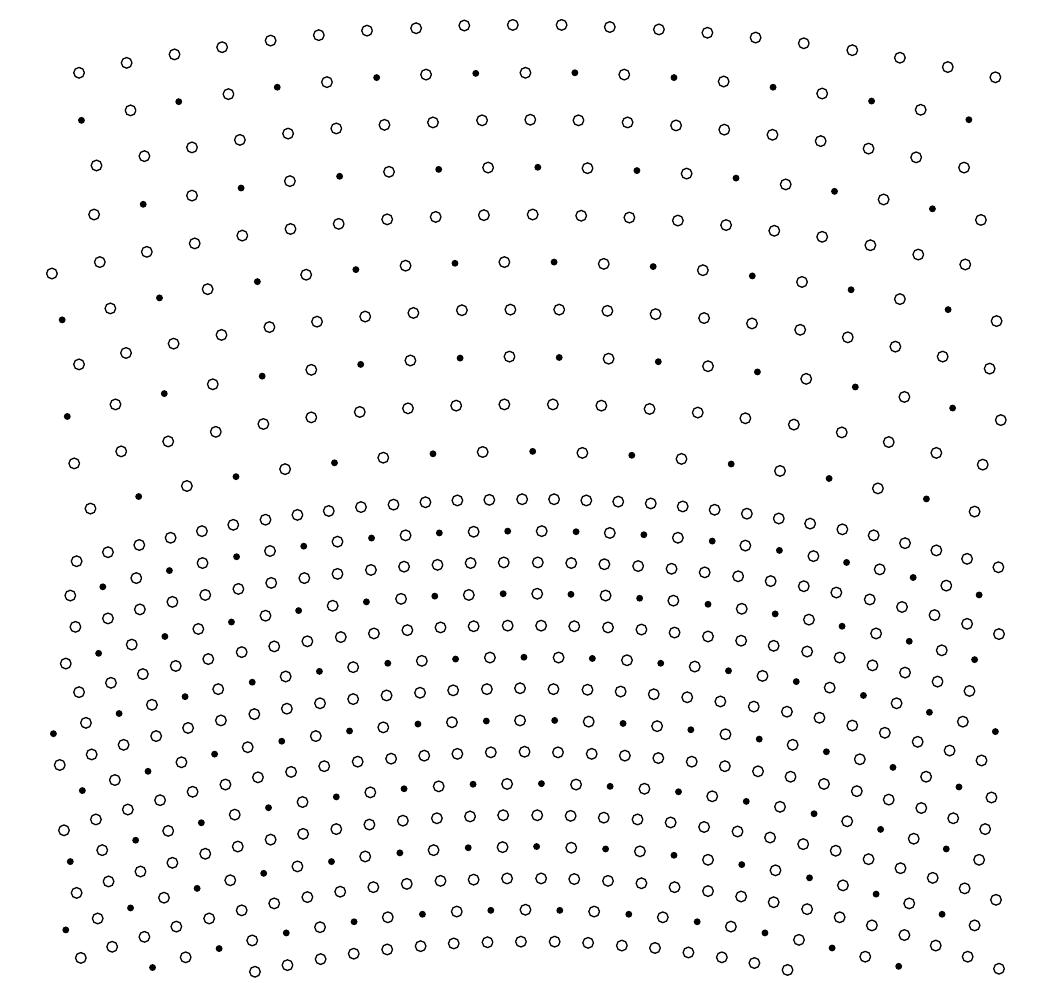
\includegraphics[height=31ex]{Chapter3_detectors/img/dc_cells}
  \hspace{1em}
  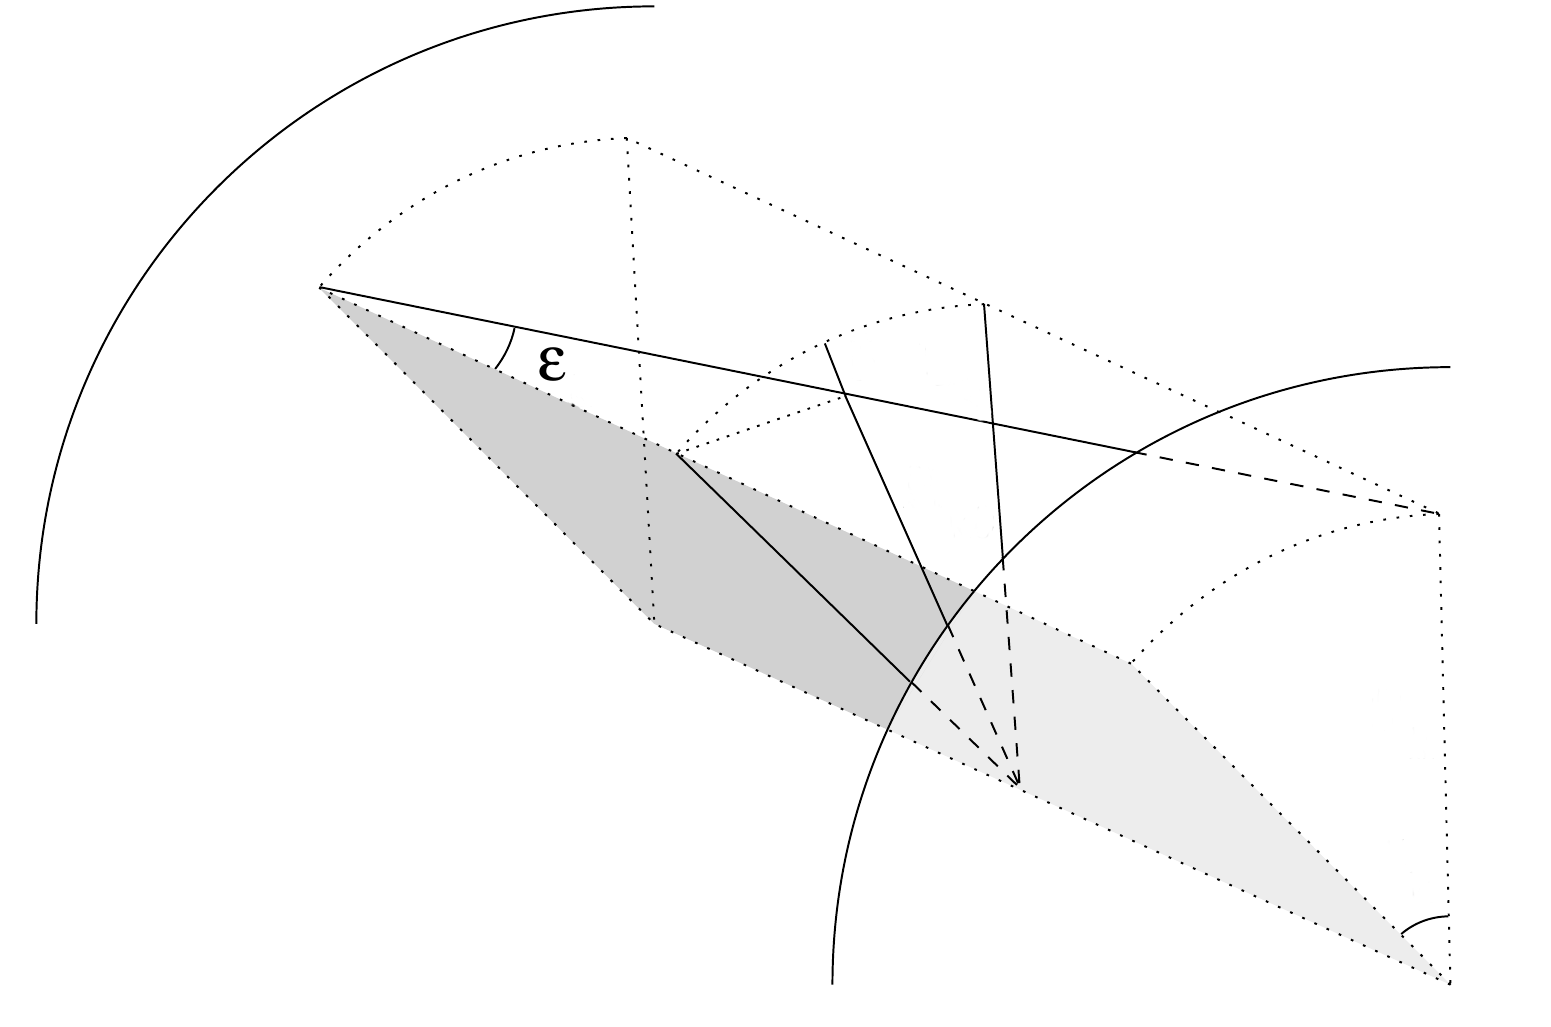
\includegraphics[height=31ex]{Chapter3_detectors/img/stereoangle1}
  \caption{Left: structure of wires and cells in a polar slice of the drift chamber. Field wires are denoted with open circles and dots indicate sense wires. Right: geometry of a wire in the KLOE Drift Chamber, mounted so as to deviate from the direction parallel to the detector $z$ axis by a small angle $\varepsilon$ in order to allow for determination of ionizing particle interaction location on the $z$ axis. Both figures were adapted from~\cite{Adinolfi:2002uk}.\label{fig:dc}}
\end{figure}

A total of almost 40000 field wires are stretched between end plates of the chamber to form electric field in the drift cells, each of which is defined  along a sense wire. The wire and cell structure of the DC shown in~\fref{fig:dc} (left) was dictated by the fact that due to small momenta of $\phi$ decay products, the track density at KLOE is higher close to the interaction point. Therefore the cells are organized radially in 58 layers, with the 12 innermost layers constituted by small 2$\times$2~cm$^2$ cells and the remainder by larger 3$\times$3~cm$^2$ cells~\cite{Adinolfi:2002uk}.
While position of gas ionization by a charged particle in the transverse ($xy$) plane is determined using spatial location of a certain sense wire and the space-time relation for particular drift cell, localization of the interaction along the $z$ detector axis is obtained with a stereo geometry of the wires, presented schematically in the right panel of~\fref{fig:dc}. In this geometry, the angle $\varepsilon$ between a wire and the chamber axis ranges between $\pm$60~mrad and $\pm$150~mrad whereas its sign alternates between subsequent layers, which ensures high and uniform coverage of the detector sensitive volume~\cite{Adinolfi:2002uk}.

Reconstruction of charged particle tracks uses information on wire geometry, external magnetic field and space-time relations for drift cells and comprises three steps: pattern recognition, track fitting and vertex fitting. The resulting spatial resolution of the KLOE drift chamber is below 200~$\mu$m in the transverse plane and 2~mm along the $z$ axis. Decay vertices, determined on the basis of closest approach of two tracks, are resolved up to 1~mm~\cite{Adinolfi:2002uk}. Finally, the momentum is attributed to a registered track using its curvature caused by the external magnetic field, yielding a relative momentum resolution at a level of \SI{0.4}{\percent}~\cite{kloe_results}. A comprehensive description of the KLOE DC reconstruction procedures can be found in Reference~\cite{data_handling}.

\subsection{The electromagnetic calorimeter of KLOE}
\label{sec:emc}
In order to cover almost the full (\SI{98}{\percent}) solid angle around the interaction point and record interactions of both photons and mesons in the energy range between 20 and 510~MeV, the KLOE electromagnetic calorimeter was built in a sampling technology using lead foils alternated with scintillating fibers of 1~mm diameter. The latter are shaped so as to enable light propagation in a single mode, thus allowing for excellent timing resolution. A single module of the EMC is composed of 200 layers of lead foil and 200 layers of fibers glued with epoxy in a lead:fiber:epoxy ratio of 42:48:10. Such composition ensures a good energy resolution due to high scintillator content. The radiation length in the calorimeter material is about 1.5~cm and the total thickness of the calorimeter amounts to about 15~radiation lengths~\cite{Adinolfi:2002zx}.

\begin{figure}[h!]
  \centering
  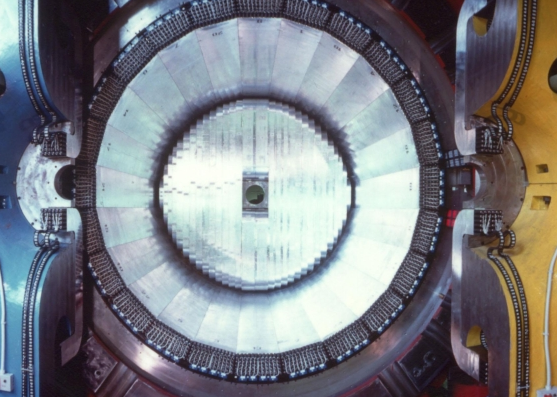
\includegraphics[height=27ex]{Chapter3_detectors/img/emc2}
  \hspace{1em}
  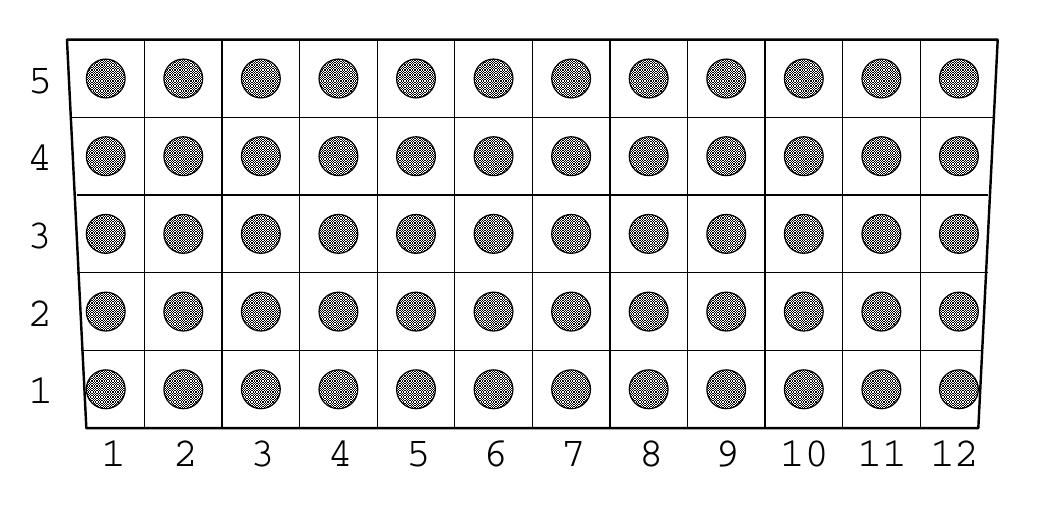
\includegraphics[height=17ex]{Chapter3_detectors/img/emc_module}
  \caption{Left: view inside the KLOE calorimeter through one of the endcaps (the other endcap is already closed). Structure of the 24 modules of the EMC barrel is visible. Figure adapted from~\cite{kloe_web}. Right: structure of EMC cells in a single barrel module with 12 columns and 5 layers. Black circles represent photomultiplier locations, each of which determined a single cell. Figure adapted from~\cite{zdebik_mgr}.}
  \label{fig:emc}
\end{figure}

The barrel part of the calorimeter is composed of 24 modules of trapezoidal cross section, located at different azimuthal angles and spanning the whole length of the barrel, as visible in the photograph in the left panel of~\fref{fig:emc}. Each of these modules is read out at both ends by photomultipliers attached through light guides and organized in a grid presented schematically in~\fref{fig:emc} (right). Each volume of a single module read out by a separate photomuliplier constitutes a distinct cell of the calorimeter, i.e.\ the smallest entity in which and energy deposition in the EMC can be localized in the transverse plane. Each cell in a module is identified by its coordinates: layer (1--5) and column number (1--12). Such segmentation of the readout results in a $xy$ resolution of energy deposition point of about 1.3~cm~\cite{Adinolfi:2002zx}. Each of the EMC endcaps consists of 32 similarly structured modules, although these modules are bent at the edges in order to position the photomultipliers parallel to the magnetic field~(see~\fref{fig:kloe}) and oriented vertically. Segmentation of the readout similar as in the barrel modules allows for position determination in the $xz$ plane in case of the endcaps.

The position of energy deposit along the calorimeter modules $s$ (w.r.t.\ center of the module) and time of interaction $t$ are estimated using the times of light registration at both ends of the modules, $t^A$ and $t^B$ (neglecting known time offsets originating from hardware):
\begin{eqnarray}
  \label{eq:emc_ts}
  s & = & \frac{\upsilon(t^A-t^B)}{2}, \label{eq:emc_s}\\
  t & = & \frac{t^A+t^B}{2} - \frac{L}{2\upsilon}, \label{eq:emc_t}
\end{eqnarray}
where $L$ denotes the length of the module and $\upsilon$ is the velocity of light propagation in the scintillating fibers~\cite{Adinolfi:2002zx}. The deposited energy is obtained from a mean of energies recorded at both ends of the calorimeter cell, measured through photomultiplier signal amplitudes corrected for light attenuation in the scintillating fibers.

As a result of the above scheme, the resolutions of energy, time and $z$ coordinate of interaction exhibit a dependence on the deposited energy, which can be approximated by the following relations~\cite{Adinolfi:2002zx}:
\begin{eqnarray}
  \label{eq:emc_res}
  \sigma(E) & = & \frac{0.057\:E}{\sqrt{E(GeV)}}, \\
  \sigma(t) & = & \frac{54\:ps}{\sqrt{E(GeV)}} \oplus 140\:ps, \\
  \sigma(z) & = & \frac{1.2\:cm}{\sqrt{E(GeV)}}.
\end{eqnarray}

After energy depositions in single cells are recorded, an algorithm searching for groups of spatially-adjacent cells with deposited energy is applied in order to identify sets of cells corresponding to a single particle interaction~\cite{data_handling, zdebik_mgr}, commonly referred to as \textit{calorimeter clusters}. The time and location of the physical interaction corresponding to a cell cluster is calculated as an energy-weighted average of member cell properties.

The excellent time resolution of the KLOE EMC for registration of photons from the $\Kl\to 3\pi^0$ process is one of the key factors allowing for a trilateration-based reconstruction of this decay described in this work. Moreover, even though the calorimeter was designed to record energy depositions starting from 20~MeV, it has proven capable of detecting photons of energies as low as 7~MeV~\cite{difalco_phd}. 

\subsection{The trigger system}\label{sec:trigger}
The trigger of the KLOE data readout is designed to accept a broad range of processes while discriminating mostly the machine background and the Bhabha $e^+e^-$ scattering. It operates on local energy deposits in the electromagnetic calorimeter and multiplicity of signals from drift chamber wires. In order to assure minimal readout delay, the trigger is divided into two levels with level 1 requiring at least one of the following:
\begin{itemize}
\item energy deposit larger that 50~MeV in the EMC barrel,
\item energy deposit larger that 150~MeV in the EMC endcaps,
\item 15 hits registered by the DC within a time window of 250~ns from a bunch crossing.
\end{itemize}
Moreover, at this level, the $e^+e^-\to e^+e^-$ events are identified by presence of clusters in the EMC with~E$>$350~MeV and are mostly rejected with only a pre-defined fraction preserved for detector calibration and accelerator luminosity monitoring. The level~1 trigger initiates early conversion of signals by the front-end electronics. However, in order to account for the full response of the drift chamber, the readout of its front-end electronics is extended to about 2~$\mu$s which corresponds to maximum drift time of electrons in the DC cells. Only then does the second trigger level process the DC-based event information along with more advanced topological requirements on the energy deposits in the calorimeter in order to validate the level 1 trigger. At level 2, a cosmic ray veto is also applied which rejects events with two $>$30~MeV energy deposits in the outer layer of the EMC\@.

As the $\Kl$ mesons at KLOE propagate in the detector with average $\beta\approx0.22$, their decays can occur tens of nanoseconds after their creation. Therefore, the trigger cannot be directly synchronized with each bunch crossing of DA$\Phi$NE\@. Instead, the readout is phase-locked to a demultiplied RF clock of the collider with a period of 4 bunch crossing ($t_{sync}=10.85$ ns)~\cite{data_handling}. The association of a recorded event to a particular bunch crossing number $N_{BC}$, is thus performed in the offline analysis in order to determine the event start time $T_0=N_{BC}\cdot T_{RF}$ ($T_{RF}=2.72$ ns), which must then be subtracted from all the times measured in the event. A first approximation of $T_0$ is obtained using the assumption that the first recorder calorimeter cluster was created by a prompt photon originating at the primary interaction point. The following relation is used to extract $T_0$ from the measured cluster time $T_{clu}$ and path length $R_{clu}$ travelled by the supposed photon to this cluster (electronics-related delays are neglected here for clarity)~\cite{data_handling}:
\begin{equation}
  T_0 = \text{nint}\footnote{nint(x) denotes the nearest integer for a real value x.} \left(\frac{T_{clu} -R_{clu} / c}{T_{RF}} \right) T_{RF}.
  \label{eq:t0_prompt}
\end{equation}
%%% @TODO: replace 'one of the further chapters' by proper subsection reference 
For events where no prompt photons are present, start time is estimated using other techniques considering flight time of heavy particles. A case of $T_0$ estimation for $K_{S}\to\pi e \nu$ events relevant for this work will be described in detail in~\sref{sec:t1_tof}.

\subsection{Background filters and data streaming}\label{sec:streaming}
Before tracking algorithms are applied to the recorded DC information, an additional background filter FILFO\footnote{\textit{FILtro di FOndo}, Italian for \textit{Background Filter}} is used for early reduction of the amount of present background to minimize the CPU time needed for event tracking. FILFO is dedicated to remove machine background relying solely on information from the electromagnetic calorimeter~\cite{data_handling}.

After complete reconstruction, a single event is assigned to one or more categories referred to as \textit{event streams} based on topological criteria. Streams constitute sets of event candidates for particular physical analyses. The following streams are used at KLOE:
\begin{itemize}
\item charged kaons,
\item neutral kaons,
\item $\phi\to\pi^+\pi^-\pi^0$ events,
\item radiative $\phi$ decays,
\item Bhabha scattering events,
\item unclassified events.
\end{itemize}
The last category contains a fraction (1/20) of all events before classification and is therefore useful for evaluation of the efficiency of event assignment to particular streams. Details of criteria on event topology required for each of the streams can be found in Reference~\cite{memo_225}.  

% @TODO: move this to analysis section
% Although all of the background rejection mechanisms described in this and the previous section are optimized to impose only minimal reduction of the physics processes of interest in KLOE, an analysis of the data collected by this setup requires accounting for finite selection efficiencies of the following filtering stages:
% \begin{itemize}
% \item cosmic ray veto,
% \item FILFO background filter,
% \item event assignment to the stream used in the analysis.
% \end{itemize}

\subsection{Detector upgrade for the KLOE-2 experiment}\label{sec:kloe2}
The KLOE detector operated in two periods, in the years 2000--2001 and 2004--2005, collecting datasets of $\phi$ decays amounting to about 450 nb$^{-1}$ and 1.7 fb$^{-1}$, respectively. Although the data analysis reported on in this Thesis was conveyed using the 2004--2005 data, an important objective of this work was to prepare tools for selection and reconstruction of relevant events, which can be applied in a future analysis of a larger dataset to be collected by the KLOE-2 experiment. KLOE-2 is constituted by the KLOE detector which has been upgraded with new components, comprising a novel inner tracking device created in the cylindrical-GEM (Gas Electron Multiplier) technology~\cite{kloe_inner_tracker} and filling the volume between the spherical beam pipe and inner wall of the drift chamber, as well as new crystal calorimeters covering in the final focusing regions of the beam~\cite{Cordelli:2013mka}, and upgraded QCAL calorimeters~\cite{Cordelli:2009xb}.

In addition to detector improvements, in particular enhanced tracking resolution due to the new inner tracker, the KLOE-2 experiment is expected to collect a larger dataset thanks to a new interaction scheme of the DA$\Phi$NE collider allowing for a higher instantaneous luminosity~\cite{Zobov:2007xw}. At the moment of writing of this Thesis, the KLOE2 experiment was in the course of its datataking with a goal to collect an integrated luminosity of at least 5 fb$^{-1}$. Reference~\cite{kloe2_general} contains a comprehensive description of the KLOE-2 physics programme.

\section{The J-PET detector}\label{sec:jpet}
The J-PET (Jagiellonian Position Emission Tomograph) is a photon detector constructed entirely at the Jagiellonian University in Krak\'ow and designed for registration of photons from electron-positron annihilations as well as decays of positronium exotic atoms. J-PET was built with a two-fold purpose in mind: as a prototype of a novel design of a Positron Emission Tomography (PET) scanner for medical imaging~\cite{moskal_patent} and for basic research, including tests of discrete symmetries in the decays of ortho-positronium states~\cite{moskal_potential}.

The detector is constituted by a total of 192 strips of plastic scintillator (EJ-230) arranged in three concentric layers which form a barrel geometry as shown in the left panel of~\fref{fig:jpet_detector}. Each scintillator strip has a length of 50~cm and rectangular cross-section with dimensions of 7$\times$19~mm$^2$ and is oriented along the barrel axis. Both ends of each scintillator strip are optically coupled with separate photomultiplier tubes (PMTs).

\begin{figure}[h!]
  \centering
  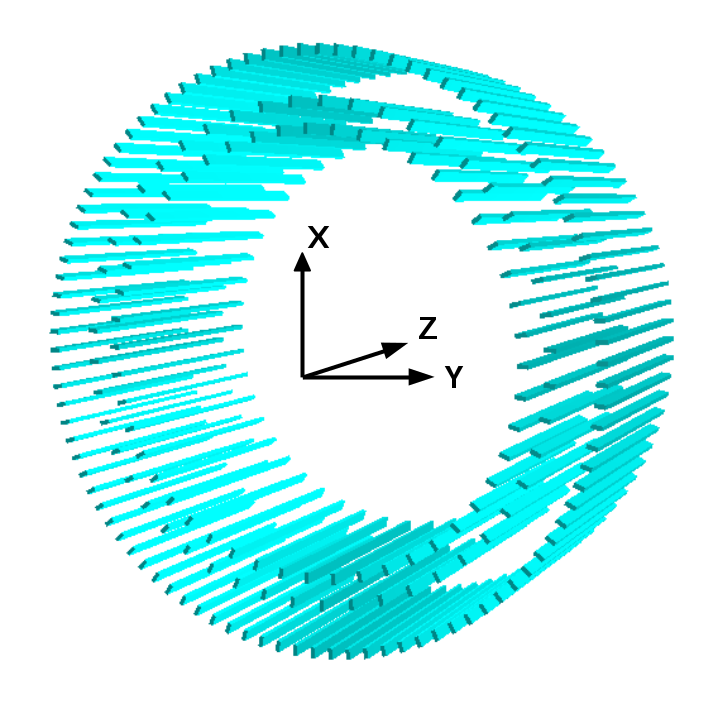
\includegraphics[width=0.4\textwidth]{Chapter3_detectors/img/pet3dxyz}
  \hspace{1em}     
  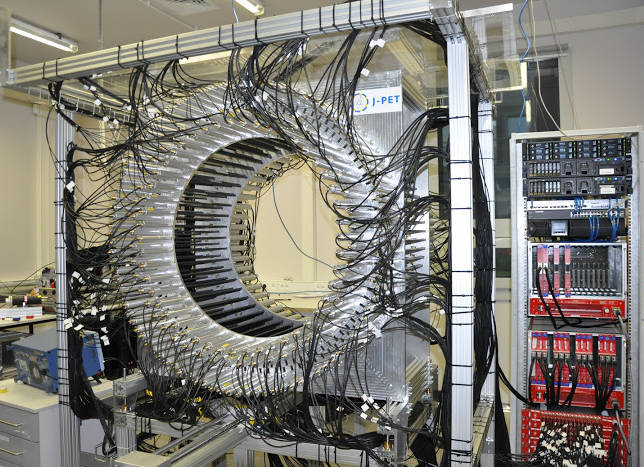
\includegraphics[width=0.5\textwidth]{Chapter3_detectors/img/pet_lab} 
  \caption{Left: arrangement of the scintillator strips constituting the J-PET detector barrel in three concentric layers and the J-PET coordinate system. There are 48 strips in each of the two innermost layers and 96 strips in the outer layer. The strips are oriented along the Z axis whereas the X direction is vertical. Right: photograph of the J-PET detector and DAQ setup. The scintillator strips (covered with black foil) are mounted between two metal plates while the photomultipliers attached to strips' ends are located outside the plates.}\label{fig:jpet_detector}
\end{figure}

Plastic scintillators used in J-PET offer fast signals with a decay time of about 1.5~ns thus allowing for a high time resolution and for use of high-activity sources~\cite{gajos_gps}. However, due to their composition mostly of elements with a low atomic number, probability of photon interaction through the photoelectric effect is negligibly small for this material. Therefore, $\gamma$ detection in J-PET is based on Compton scattering instead. A photon scattered in a plastic scintillator strip transfers a fraction of its energy to the scattered electron whose further interactions in the material lead to production of photons from the visible light spectrum~\cite{anna_scints}. The sides along a scintillator strip are covered with reflective foil to ensure total internal reflection of these photons, which leads to their propagation to the two ends of the strip with losses only due to light attenuation in the scintillator. The ends of the strip are optically connected to the windows of \mbox{PMT-s} which collect photons produced in the $\gamma$ interaction and transform them into electric signals.

\begin{figure}[h!]
  \centering
  \begin{tikzpicture}[
  scale=0.4
  ]
  \definecolor{scint}{rgb}{0.12, 0.56, 1.0}
  \definecolor{metal}{rgb}{0.75, 0.75, 0.75}
  \coordinate (interaction) at (-2,0);
  % scint
  \draw[fill, scint] (-7,-0.7) -- (-7,0.7) -- (7,0.7) -- (7,-0.7);
  % pmts
  \draw[fill, metal] (7,-1.2) -- (7,1.2) -- (11,1.2) -- (11,-1.2) node[black] at (9,0) {\large PMT B};
  \draw[fill, metal] (-7,-1.2) -- (-7,1.2) -- (-11,1.2) -- (-11,-1.2) node[black] at (-9,0) {\large PMT A};;
  % z = 0
  \draw[black, line width=1, dashed, dash pattern=on 7pt off 4pt] (0,1.5) -- (0,-2) node[right] {\Large $z=0$};
  % interaction
  \draw[black, line width=1, dashed] (-2,0) -- (-2,3);
  \node[black, above] at (-2,3) {\large $t_{\gamma}$};
  \node[star,star points=10, inner sep=0.1cm, draw, thick, fill=red!100] at (interaction) {};
  % time arrows
  \draw[line width=1.5, black, <->] (-7,2) -- (-2,2) node[midway, above] {\large $s_{A}$};
  \draw[line width=1.5, black, <->] (-2,2) -- (7,2) node[midway, above] {\large $s_{B}$};
  \draw[snake it, red, thick, ->] (0,4) -- (-1.75,0.4);
  \end{tikzpicture}
  \caption{Determination of the $z$ coordinate of a $\gamma$ interaction point (red star) in a J-PET scintillator strip (blue). Position along the scintillator is calculated as a difference of the $s_A$ and $s_B$ paths travelled by scintillation light along the strip from the interaction point to the photomultiplier tubes, obtained from the PMT signal arrival times and effective velocity of light in the scintillator.} \label{fig:jpet_strip}
\end{figure}

In terms of reconstruction of the time and place of particle interactions, the J-PET detector shares several similarities with the electromagnetic calorimeter of KLOE described in~\sref{sec:emc}. While position of a $\gamma$ interaction point in the XY plane of the detector is determined up to the location of a single scintillator (which corresponds to an azimuthal angle resolution at the level of 1 degree~\cite{gajos_gps}), the Z coordinate of the interaction is inferred from the difference between times of light propagation to both ends of the scintillator strip as shown in~\fref{fig:jpet_strip}. While exact time needed by the optical photons to travel from the interaction point to a strip end depends on a particular sequence of internal reflections, the average light propagation along the strip can be described by an effective velocity $\upsilon_{e}$, determined as a calibration constant of the detector~\cite{jpet_single_module}. Assuming the $\gamma$ was scattered in the scintillator at time $t_{\gamma}$, the times of light arrival to the two ends of the strip (labeled A and~B) $t_A$ and $t_B$ can be expressed as:
\begin{eqnarray}
  \label{eq:jpet_zpos}
  t_A &=& t_{\gamma} + \frac{s_A}{\upsilon_{e}},\\
  t_B &=& t_{\gamma} + \frac{s_B}{\upsilon_{e}}.
\end{eqnarray}
The interaction position along the $z$ axis, measured with respect to the strip center, is proportional to the difference of the light registration times at PMT-s A and B and is thus obtained using the same formula as in case of the KLOE electromagnetic calorimeter (compare~\eref{eq:emc_s}):
\begin{equation}
  \label{eq:jpet_zpos2}
  z_{\gamma} = \frac{s_A - s_B}{2} = \frac{\upsilon_{e}\left( t_A - t_B \right)}{2}.
\end{equation}
Similarly, the time of the interaction $t_{\gamma}$ can be obtained from a sum of the light registration times at sides A and B of the scintillator, again using the same recipe in the KLOE EMC (compare~\eref{eq:emc_t}):
\begin{equation}
  \label{eq:jpet_hittime}
  t_{\gamma} = \frac{t_A + t_B}{2}  - \frac{L}{2\upsilon_{e}},
\end{equation}
where $L=s_A+s_B$ is the length of the scintillator strip.

The majority of $\gamma$ interactions in the plastic scintillators are through Compton scattering, where amount of energy deposited by the incident $\gamma$ depends on the scattering angle with a differential cross-section for scattering in a solid angle element d$\Omega$ given by the Klein-Nishina formula~\cite{Griffiths}:
\begin{equation}
  \label{eq:klein_nishina}
  \frac{\text{d}\sigma}{\text{d}\Omega} = \frac{r_0^2}{2}\left(\frac{E'}{E}\right)^2\left[ \frac{E}{E'} + \frac{E'}{E} - sin^2\vartheta \right],
\end{equation}
where $r_0$ is the classical electron radius, $E$ and $E'$ denote energies of the primary and scattered photon and $\vartheta$ is the planar angle between their momenta.

What follows is that a scattered photon can deposit any energy from a continuous spectrum between zero and a certain boundary value smaller than its total energy. This maximal transferred energy, corresponding to $\gamma$ back-scattering, smeared by experimental effects constitutes a characteristic cut-off in the spectrum, referred to as the Compton edge. \fref{fig:compton} presents exemplary simulated energy deposition spectra for three different energies of incident $\gamma$~quanta, where different positions of Compton edges are visible. Consequently, although it is impossible to measure the photon energy directly through registration of a single interaction, $\gamma$ quanta of energies significantly larger than annihilation products can be distinguished by the amount of deposited energy above the Compton spectrum edge for 511~keV photons.

\begin{figure}[h!]
  \centering
  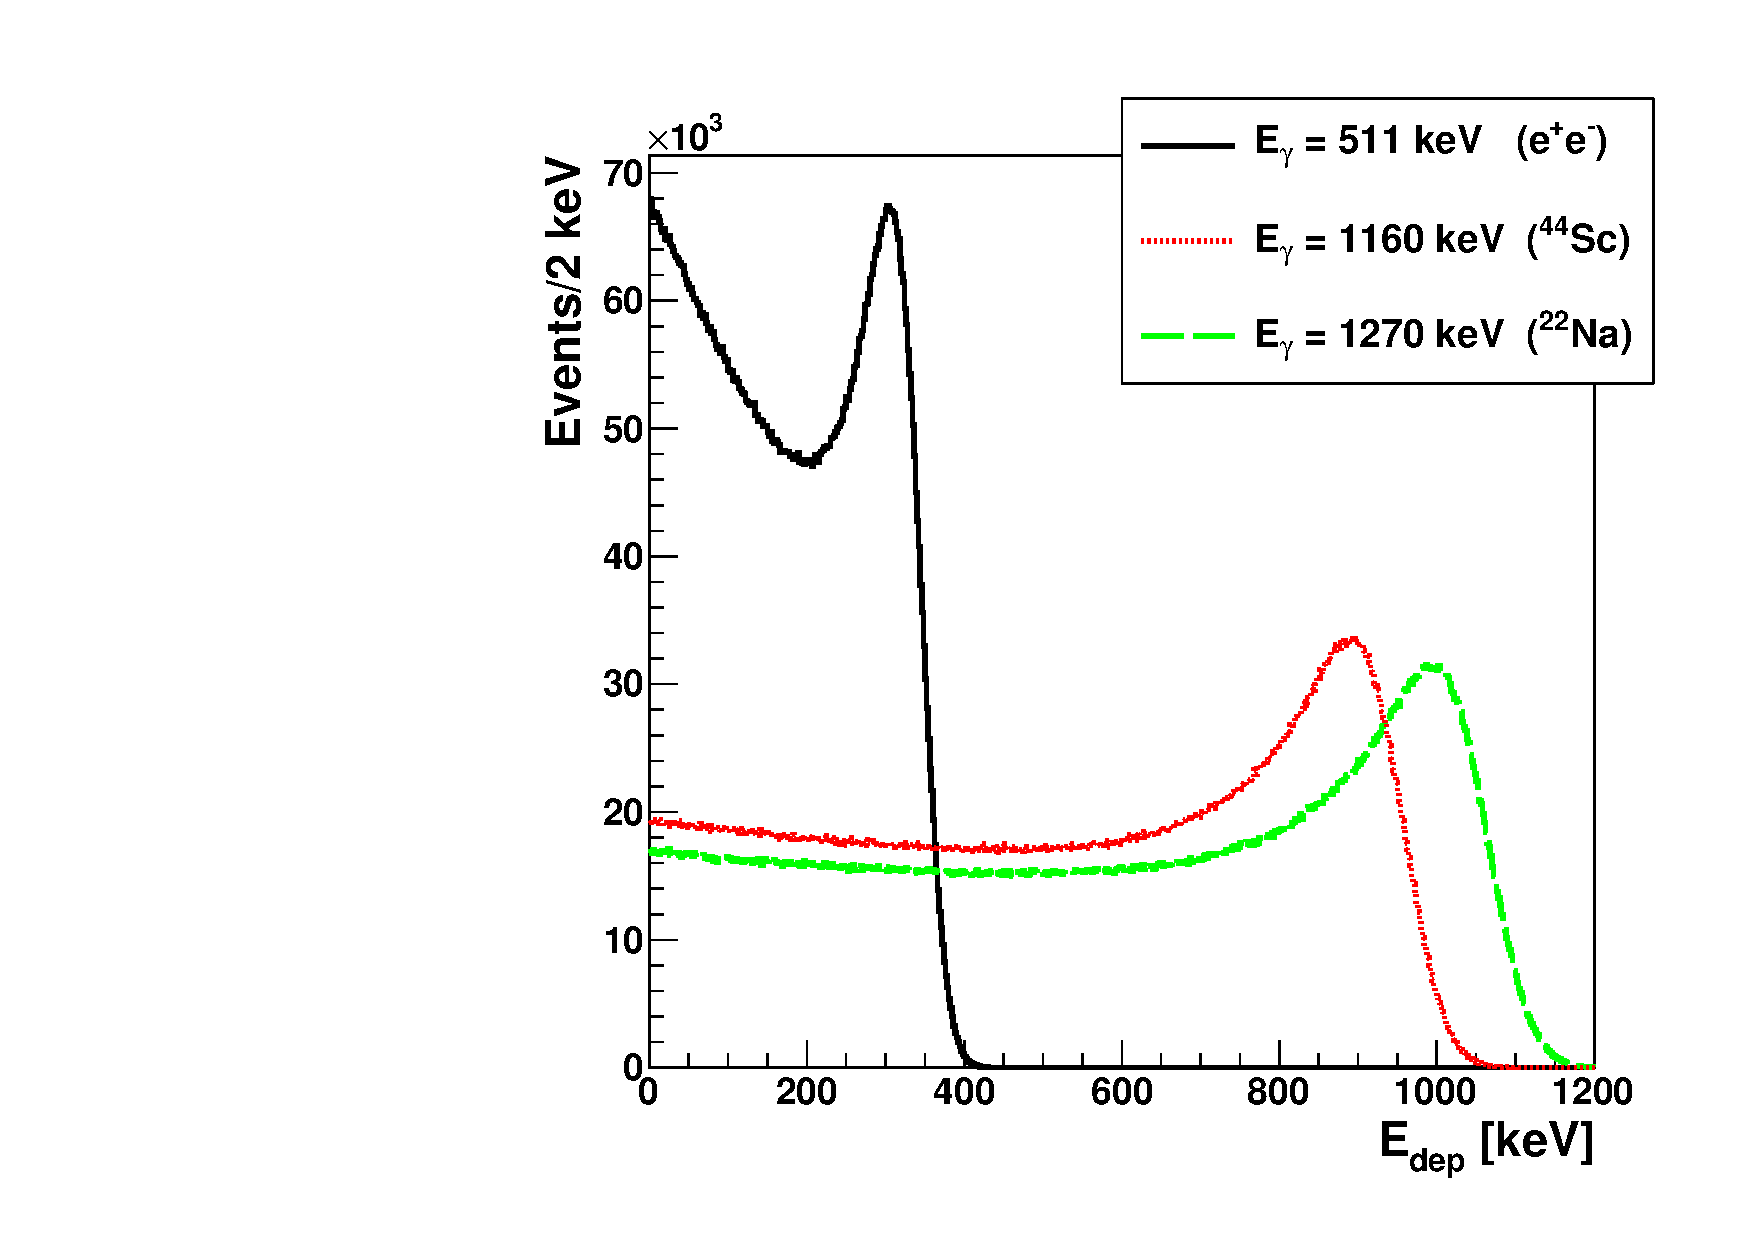
\includegraphics[width=0.5\textwidth]{Chapter3_detectors/img/compton}
  \caption{Simulated energy deposition spectra for Compton scattering of $\gamma$ with various energies in the J-PET plastic scintillators. Figure was adapted from~\cite{daria_epjc}.}
  \label{fig:compton}
\end{figure}

J-PET therefore attempts to measure the deposited energy indirectly through estimation of an integral of electric signals produced by the PMT-s in response to the recorded scintillation light. This estimation is based on the time-over-threshold (TOT) measurement enabled by dedicated front-end electronics (FEE)~\cite{marek_fee}. The J-PET front-end electronics are connected to the photomultiplier tubes which produce negative electric signals (understood as voltage changes in time). The FEE probe electric signals in the time domain at four preset threshold values of voltage $\upsilon_i, \: i=1,\ldots,4$ as depicted in~\fref{fig:jpet_signal}. For each of the threshold voltages, the FEE output a logical signal at the moment when the signal voltage crosses the threshold, separately for the leading and trailing edge of the signal~\cite{marek_fee}. These logical signals are passed to the Time-to-Digital Converters (TDC-s) of the data acquisition (DAQ) system~\cite{greg_daq} which produces up to 8 timestamps per a single PMT signal. Times recorded for both the leading and trailing signal edge at the same threshold $i$ may be used to calculate the time-over-threshold value:
\begin{equation}
  \label{eq:tot_i}
  TOT_i = t^T_i-t^L_i.
\end{equation}
A set of $TOT_i$ values at certain thresholds constitute a measure of the signal size (understood as its the integral, compare~\fref{fig:jpet_signal}), the sum of TOT-s at all thresholds crossed by the signals on both A and B sides of a scintillator allow for an estimation of the energy deposited in the strip by a $\gamma$ quantum. In further considerations, such a sum of TOT values will be referred to as TOT for a certain $\gamma$ interaction recorded in J-PET:
\begin{equation}
  \label{eq:tot_def}
  TOT_{\gamma} = \sum_{i=1}^4 TOT_i^{A} + \sum_{i=1}^4 TOT_i^{B}.
\end{equation}

\begin{figure}[h!]
  \centering
  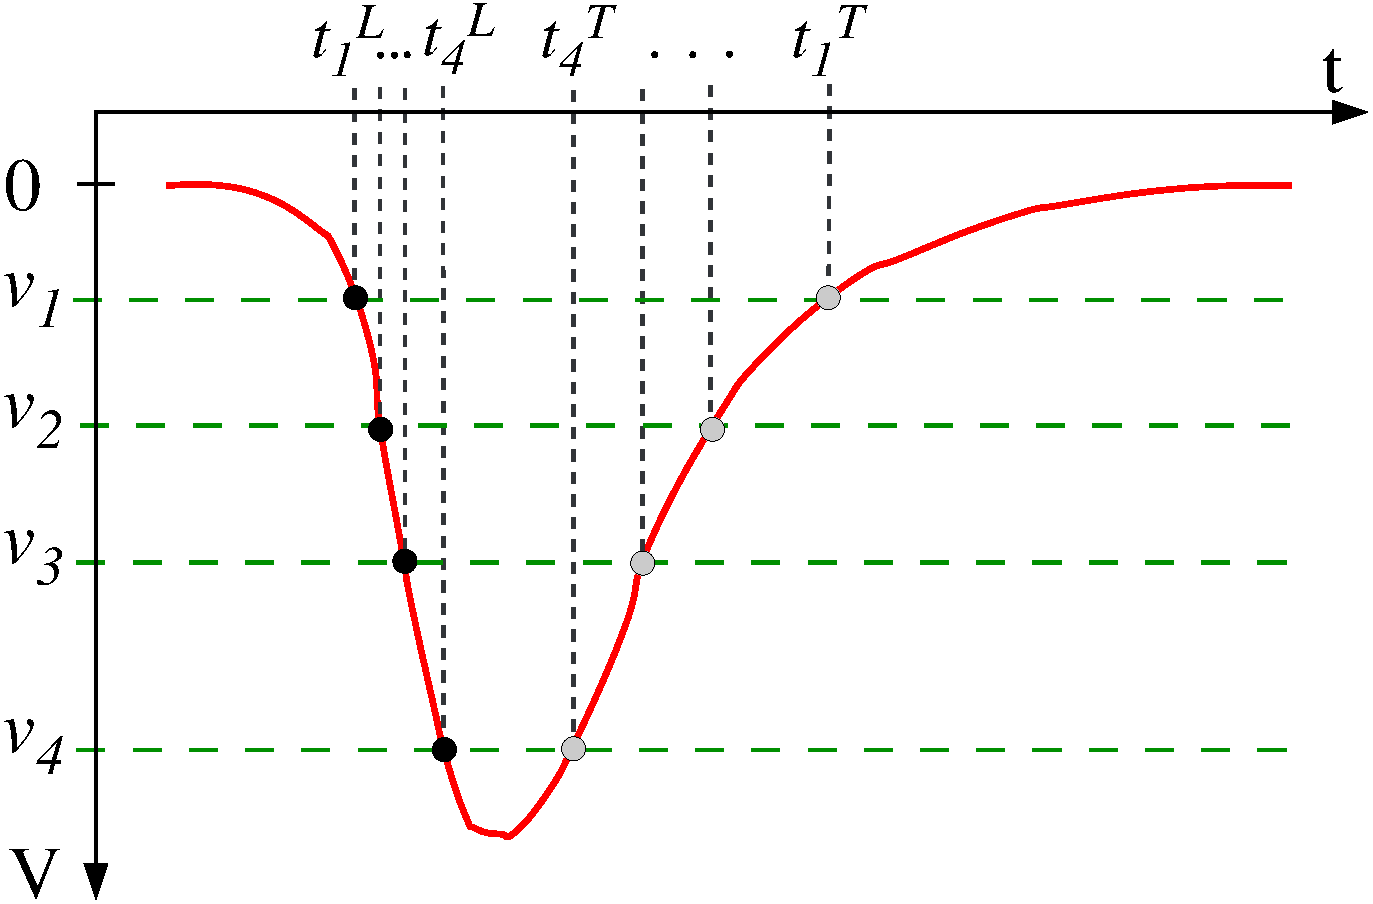
\includegraphics[width=0.6\textwidth]{Chapter3_detectors/img/jpet_sig2}
  \caption{Scheme of digitalization of a photomultiplier signal by the J-PET front-end electronics. An electric signal (red) is sampled at four preset voltage threshold levels
(green) $\nu_{i}, \ i=1,\ldots,4$. Times of the signal voltage crossing the thresholds are recorded at both leading ($t_i^{L}$) and trailing edge ($t_i^{T}$) of the signal (black and gray dots respectively).}\label{fig:jpet_signal}
\end{figure}

In addition to providing a measure of deposited energy, this signal digitalisation scheme allows for a partial retrieval of the original signal shape based on the recorded points with techniques such as compressive sensing~\cite{lech_compressive}. Moreover, it provides additional information on the signal leading edge useful for precise reconstruction of its arrival time, needed in turn for determination of the interaction $z$ position using relations~\ref{eq:jpet_zpos2} and~\ref{eq:jpet_hittime}. A more advanced approach to the logitudinal interaction position reconstruction has also been studied with a simplified J-PET prototype~\cite{neha_synchronized}.

Since any non-trivial reconstruction preformed in the J-PET detection 
is based on measurements of times, 
calibration of the recorded time values is crucial for the obtained accuracy. Time calibration is performed with a point-like source of annhilation photon pairs coupled with small auxiliary reference detector approaching subsequently every scintillator strip and positioned precisely at its center in order to provide reference events for which $t_A=t_B$. A detailed description of the time calibration procedure can be found in~\cite{jpet_time_calibration}.
Although the exact resolution of the time and $z$ position determination of $\gamma$ scattering in J-PET is only under study at the moment of writing of this Thesis, studies involving a two-dimensional prototype of the same design have shown that the achievable resolution can be as low as $\sigma(t_{\gamma}) = 80$ ps and  $\sigma(z_{\gamma}) = 0.93$ cm~\cite{jpet_single_module}.

\subsection{Polarization control}\label{sec:ops_polarization}
Calculation of the angular correlation operators described in~\cref{chapter:test_jpet} relies on determination of the spin of decaying ortho-positronia. With an appropriate experimental setup presented schematically in~\fref{fig:ops_spin_determination}, this can be performed on an event-by-event basis to an extent limited by several statistical factors. In the planned setup, a $\beta^+$ radioactive point-like source will be placed in the center of a cylindrical vacuum chamber whose walls will be coated on the inner side with a porous medium for \ops/ production. Certain materials such as silica aerogels can be used as the medium to maximize the ratio of \ops/$\to 3\gamma$ to total annihilation rate and to other $3\gamma$ annihilations not originating from an ortho-positronium state~\cite{Jasinska:2016qsf,moskal_potential}. Positrons from the source, after reaching the medium on the chamber walls, undergo thermalization and may form ortho-positronium atoms. As the possible distance travelled by the \ops/ atom before its decay is negligible, reconstruction of the decay point, along with the fixed $\beta^+$ source location, allows for an estimation of the original positron flight direction (see~\fref{fig:ops_spin_determination}). Positrons from a $\beta^+$ decay are spin-polarized along their velocity vector $\vec{\upsilon}_e$ with an average polarization $\vec{P}=\frac{\vec{\upsilon}_e}{c}$ due to parity violation, therefore knowledge of the $\vec{\upsilon}_e$ direction defines the positron spin direction with an average uncertainty dependent on the mean positron energy and thus on the chosen $\beta^+$ emitter~\cite{moskal_potential}.

\begin{figure}[h!]
  \centering
  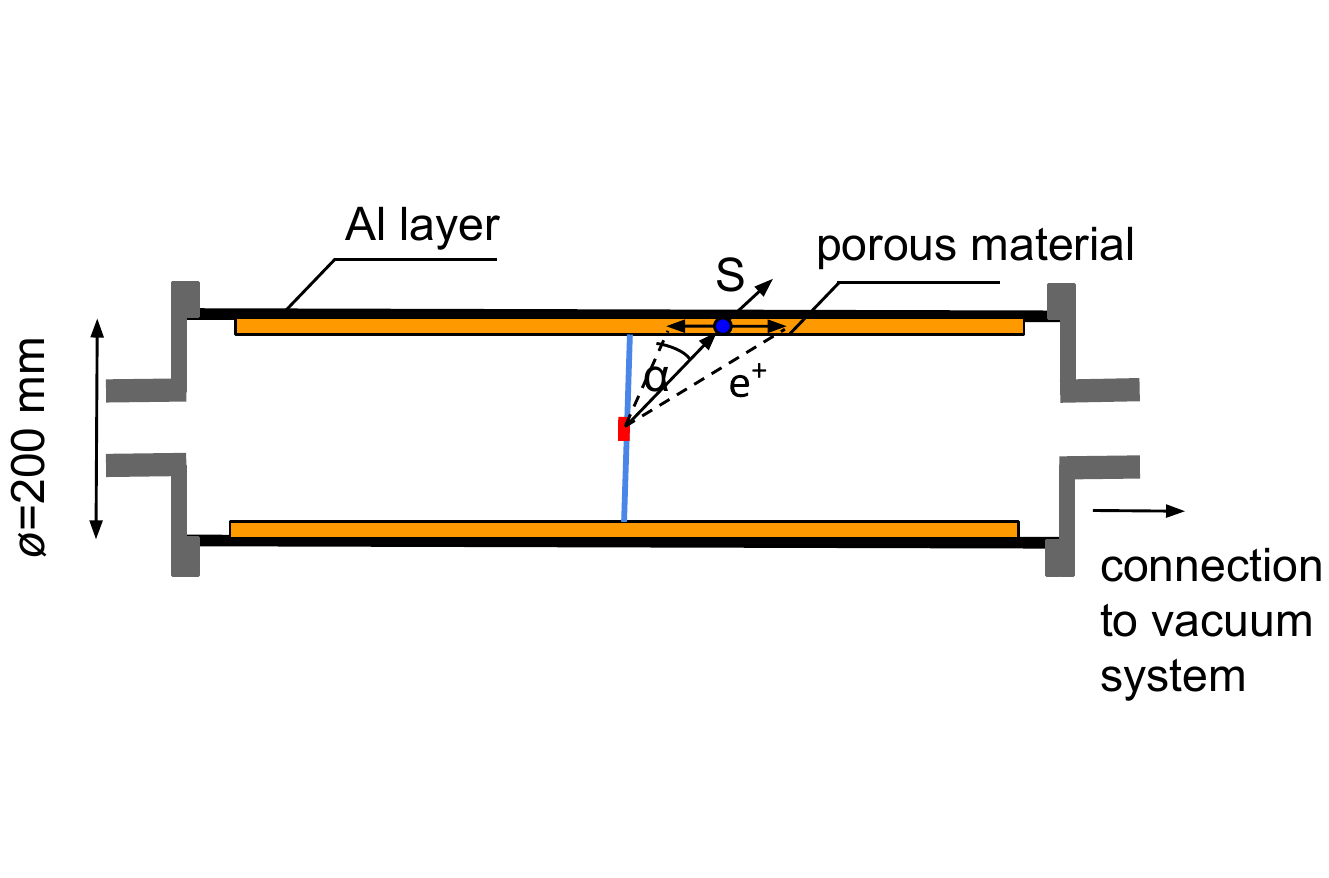
\includegraphics[width=0.6\textwidth]{Chapter5_test_jpet/img/chamber}
  \hspace{1em}
  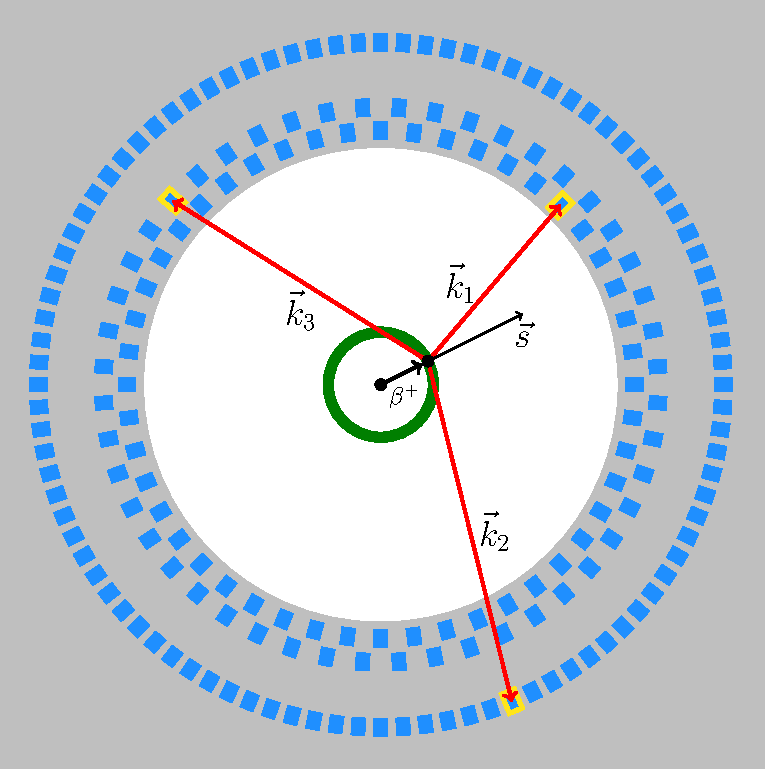
\includegraphics[width=0.35\textwidth]{Chapter5_test_jpet/img/pet-ops}
  \caption{Left: longitudinal section of an o-Ps annihilation chamber allowing for determination of ortho-positronium spin direction throught spin of the positron which creates it. Right: scheme of the o-Ps spin reconstruction in the J-PET detector presented in its transverse plane.}
  \label{fig:ops_spin_determination}
\end{figure}

The average uncertainty on the determined \ops/ spin further depends on the polarization loss during positron thermalization~\cite{PhysRevLett.43.1281} and the fact that only 2/3 of the created positronia retain the spin of the positron~\cite{Arbic:1988pv}. Moreover, an indeterminacy of the positron direction within a cone with an $\alpha$ opening angle (indicated in the left panel of~\fref{fig:ops_spin_determination}) diminishes the polarization by an additional factor of $\frac{1}{2}(1+cos(\alpha))$~\cite{Coleman}. Since the impacts of thermalization and \ops/ formation on the final spin estimation are inevitable, it is crucial to minimize the effect from positron flight direction uncertainty. This can be achieved with a precise reconstruction of the ortho-positronium annihilation point, providing which was one of the objectives of this Thesis. Next Chapter contains a description of a suitable \ops/$\to 3\gamma$ reconstruction technique whereas the results of its preliminary performance studies are presented in~\cref{chapter:analysis_jpet}.


%%%
% do zacytowania:
%%%
% rekonstrukcja \cite{neha_synchronized} \cite{lech_compressive}
% kalibracja \cite{jpet_time_calibration}
% jak zrekonstruować energie na podstawie kątów \cite{daria_epjc}
% 80ps i efektywna predkosc \cite{jpet_single_module}
% pierwsze studia odrzucania tła, suma vs roznica kątów etc. \cite{jpet_commissioning}



 	
%%% Local Variables:
%%% TeX-master: "../main"
%%% End: